\documentclass{scrartcl}
\title{\rmfamily Software Engineering -- Blatt 7}
\author{Rasmus Diederichsen \and Felix Breuninger\and 
   \texttt{\{rdiederichse, fbreunin\}@uos.de}
}
\date{\today}
\usepackage[ngerman]{babel}
\usepackage{marvosym, microtype, textcomp, xifthen, multirow, booktabs, dingbat,
   titlesec, enumitem, fullpage, tikz, IEEEtrantools, array, amsmath, listings,
amssymb, graphicx, subcaption, lmodern,pgfplots}
\usepackage[pdftitle={Software Engineering -- Blatt 7}, 
   pdfauthor={Rasmus Diederichsen, Felix Breuninger}, 
   hyperfootnotes=true,
   colorlinks,
   bookmarksnumbered = true,
   linkcolor = lightgray,
   plainpages = false,
citecolor = lightgray]{hyperref}
\usepackage[utf8]{inputenc}
\usepackage[T1]{fontenc}
\usepackage[all]{hypcap}
\titleformat{\subsection}[hang]{\bf}{Aufgabe \arabic{section}.\arabic{subsection}:}{1em}{}[]
\titleformat{\subsubsection}[hang]{\bf}{\hspace{1em}\alph{subsubsection})}{1em}{}[]

\lstset{
   frame=single,
   basicstyle=\ttfamily\small,
   frameround=tttt,
   backgroundcolor=\color{lightgray!10},
   keywordstyle=\color{teal}\textbf,
   stringstyle=\itshape,
   showstringspaces=false,
   language=[gnu] make,
   morecomment=[n]{$(}{)},
   commentstyle=\color{blue},
   title=\lstname
}
\usetikzlibrary{shapes,positioning,calc,decorations.text,graphs,arrows.meta}
\begin{document}

\fontfamily{ptm}\selectfont
\maketitle

\setcounter{section}{7}
\setcounter{subsection}{0}

\subsection{Programmablaufplan, Struktogramm}

\subsubsection*{Struktogramm}

\begin{center}
   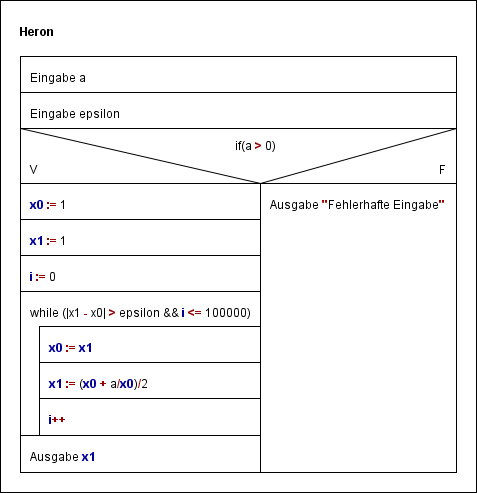
\includegraphics[scale=0.6]{Heron.png}
\end{center}

% style for PAP
\tikzstyle{typewriter} = [font=\ttfamily]
\tikzstyle{decision} = [diamond, draw, fill=blue!20, typewriter,
                        text width=4.5em, text badly centered, inner sep=0pt]
\tikzstyle{block}    = [rectangle, draw, fill=blue!10, typewriter,
                        text width=6em, text centered, minimum height=3em]
\tikzstyle{line}     = [draw, -latex', typewriter]
\tikzstyle{cloud}    = [draw, ellipse,fill=red!20, node distance=3cm,
                        minimum height=2em, typewriter]
\tikzstyle{io}       = [draw,trapezium,trapezium left angle=70,trapezium right
angle=-70,minimum height=3em]

\subsubsection*{PAP}

\begin{tikzpicture}
   \node[cloud] (begin) {Heron};
   \node[io,below=of begin] (zahl) {Zahlen a, $\varepsilon$};
   \node[decision,below=of zahl] (a>0) {A > 0 ? \&\& $\varepsilon > 0$};
   \node[io,left=of a>0] (err) {Error};
   \node[cloud,left=of err] (end) {Ende};
   \node[block,below=of a>0] (assignx0) {$x_0$ = 1};
   \node[block,below=of assignx0] (assignx1) {$x_1$ = 1};
   \node[block,below=of assignx1] (assignc) {c = 0};
   \node[block,below=of assignc] (step) {$x_1=\frac{x_0+\frac{a}{x_0}}{2}$};
   \node[block,below=of step] (c++) {c = c + 1};
   \node[decision,below=of c++] (converge) {$|x_1 - x_0| \le \varepsilon$ ?};
   \node[io,left=of converge] (finish) {Näherung: $x_1$};
   \node[decision,below=of converge] (maxiter) {c > 100000 ?};
   \node[block,right=of c++] (updatex0) {$x_0 = x_1$};

   \draw[-{Latex}] (begin) -- (zahl);
   \draw[-{Latex}] (zahl) --  (a>0);
   \draw[-{Latex}] (a>0) -- node[midway,left] {Ja} (assignx0);
   \draw[-{Latex}] (assignx0) -- (assignx1);
   \draw[-{Latex}] (assignx1) -- (assignc);
   \draw[-{Latex}] (assignc) -- (step);
   \draw[-{Latex}] (step) -- (c++);
   \draw[-{Latex}] (c++) -- (converge);
   \draw[-{Latex}] (converge) -- node[midway,right] {Nein} (maxiter);
   \draw[-{Latex}] (converge) -- node[midway,above] {Ja} (finish);
   \draw[-{Latex}] (maxiter) -| node[midway,left] {Ja} (finish);
   \draw[-{Latex}] (maxiter) -| node[midway,right] {Nein} (updatex0);
   \draw[-{Latex}] (updatex0) |- (step);

   \draw[-{Latex}] (a>0) -- node[midway,above] {Nein} (err);
   \draw[-{Latex}] (err) -- (end);
   \draw[-{Latex}] (finish) -| (end);

\end{tikzpicture}

\subsection{Strukturierte Analyse}

\subsubsection{DFD}

Siehe \autoref{üdfd}, \autoref{ba-dfd}, \autoref{proz-dfd} und \autoref{tv-dfd}.

\begin{figure}[h]
   {\centering      
      \begin{tikzpicture}[every node/.append style={draw},node distance=3cm]
         \path 
         node[rectangle] (student) {Student}
         node[rectangle,right=8cm of student] (dozent) {Dozent}
         node[ellipse,below right=of student] (anmelden) {BA anmelden}
         node[rectangle,below left=of anmelden] (prüfungsamt) {Prüfungsamt};

         \draw[-{Latex},postaction=decorate,decoration={raise=5pt, text along
         path, text={Pers. Daten}, text align=center}] (student.east)  -| (anmelden.north);

         \draw[-{Latex},postaction=decorate,decoration={raise=5pt, text along path,
         text={Wunschgebiet}, text align=center}] (student) --  (anmelden);

         \draw[-{Latex},postaction=decorate,decoration={raise=-10pt, text along path,
         text={Abgabeinfos}, text align=center,reverse path}] (anmelden) to[bend left]
         (student);

         \draw[-{Latex},postaction=decorate,decoration={raise=5pt, text along path,
         text={Ablehnung}, text align=center,reverse path}] (anmelden) to [bend right=120,looseness=1.5] (student.north);

         \draw[-{Latex},postaction=decorate,decoration={raise=5pt, text along path,
         text={Vorschlag}, text align=center, reverse path}] (dozent.south
         west) -- (anmelden.north east);

         \draw[-{Latex},postaction=decorate,decoration={raise=5pt, text along path,
         text={Anmeldebogen}, text align=center}] (anmelden.east) to[bend right]
         (dozent.south east);
         \draw[-{Latex}] (anmelden.east) to[bend right] (dozent.south east);

         \draw[-{Latex},postaction=decorate,decoration={raise=5pt, text along path,
         text={Anmeldebogen},text align=center}] (prüfungsamt) 
         -- (anmelden);

      \end{tikzpicture}
      \caption{Übersichts-DFD}
   \label{üdfd}}
\end{figure}
\tikzset{two sided/.style={
      draw=none,
      append after command={
         (\tikzlastnode.north east) edge[thick] (\tikzlastnode.north west) 
         (\tikzlastnode.south west) edge[thick] (\tikzlastnode.south east)
      }
   }
}

\begin{figure}[h]
   {\centering      
      \begin{tikzpicture}[every node/.append style={draw},node distance=3cm]
         \draw[dotted,thick,rounded corners=10pt] (-3.5cm,-5cm) rectangle (12cm,3.5cm);
         \path 
         node[ellipse] (prozedur) {Anmeldungsprozedur}
         node[ellipse,right=4cm of prozedur] (themenverwaltung) {Themenverwaltung}
         node[two sided,below=of prozedur] (opium) {OPIUM}
         node[two sided,below=of themenverwaltung] (themendb) {Themen-DB};

         \draw[-{Latex},postaction=decorate,decoration={raise=5pt, text along path,
         text={Ablehnung},reverse path, text align=center}] (prozedur.west) -- ++(-2cm,0);

         \draw[-{Latex},postaction=decorate,decoration={raise=5pt, text along path,
         text={Abgabeinfos},text align={left indent=1em}}] (prozedur.90) -- ++(0,4cm);

         \draw[-{Latex},postaction=decorate,decoration={raise=5pt, text along path,
         text={Anmeldebogen},text align={left indent=1em}}] (prozedur.20) -- ++(0,4cm);

         \draw[-{Latex},postaction=decorate,decoration={raise=5pt, text along path,
         text={Pers. Daten},reverse path,text align={left indent=1em}}] ($(prozedur.160) + (0,4cm)$) --
         (prozedur.160);

         \draw[-{Latex},postaction=decorate,decoration={raise=5pt, text along path,
         text={Thema},reverse path,text align=center}] (themenverwaltung) -- (prozedur);

         \draw[-{Latex},postaction=decorate,decoration={raise=5pt, text along path,
         text={Wunschgebiet},reverse path,text align={left indent=1em}}]
         ($(themenverwaltung.160) + (0,4cm)$) -- (themenverwaltung.160);

         \draw[-{Latex},postaction=decorate,decoration={raise=5pt, text along path,
         text={Vorschlag},reverse path,text align={left indent=1em}}]
         ($(themenverwaltung.90) + (0,4cm)$) -- (themenverwaltung.90);

         \draw[-{Latex},postaction=decorate,decoration={raise=5pt, text along path,
         text={Pers. Daten},reverse path,text align=center}] (prozedur.240) -- (opium.135);

         \draw[-{Latex},postaction=decorate,decoration={raise=5pt, text along path,
         text={Pr{\"u}fungsdaten},text align=center}] (opium.30) --
         (prozedur.320);

         \draw[-{Latex},postaction=decorate,decoration={raise=5pt, text along path,
         text={Vorschlag},reverse path,text align=center}] (themenverwaltung.240) -- (themendb.135);

         \draw[-{Latex},postaction=decorate,decoration={raise=5pt, text along path,
         text={Thema},text align=center}] (themendb.30) -- (themenverwaltung.320);

         \draw[-{Latex},shorten >=2pt,postaction=decorate,decoration={raise=5pt, text along path,
         text={Wunschgebiet},reverse path,text align=center}]
         (themenverwaltung.342) -- (themendb.10);

      \end{tikzpicture}
      \caption{Verfeinerungs-DFD für ``BA anmelden''}
   \label{ba-dfd}}
\end{figure}
\begin{figure}[h]
   {\centering      
      \begin{tikzpicture}[every node/.append style={draw,align=center},node distance=3cm]
         \draw[dotted,thick,rounded corners=10pt] (-4.5cm,-7cm) rectangle (10cm,4cm);
         \path 
         node[ellipse] (berechtigung) {Berechtigung Prüfen}
         node[ellipse,below right=1cm and 2cm of berechtigung,text width=3cm] (bogen) {Anmeldebogen erstellen}
         node[ellipse,text width=3cm,below=of berechtigung] (opium-eintrag) {OPIUM-Eintrag
         erstellen}
         node[two sided,below=of bogen] (opium) {OPIUM};

         \draw[-{Latex},postaction=decorate,decoration={raise=5pt, text along
         path, text={Ablehnung},reverse path,text align=center}] (berechtigung.north west) --
         ++(-4cm,0);

         \draw[-{Latex},postaction=decorate,decoration={raise=5pt, text along
         path, text={Abgabeinfos},reverse path,text align=center}] (berechtigung.south west) -- ++(-4cm,0);

         \draw[-{Latex},postaction=decorate,decoration={raise=5pt, text along
         path, text={Pers. Daten}, reverse path,text align=center}] ($(berechtigung.north) + (0,4cm)$) --
         (berechtigung);

         \draw[-{Latex}] ($(berechtigung.north) + (0,4cm)$) -- ++(0,-1cm) -| (bogen);

         \draw[-{Latex},postaction=decorate,decoration={raise=5pt, text along
         path, text={Anmeldebogen},text align=center}] (bogen.north east) -- ++(4cm,0);

         \draw[-{Latex},postaction=decorate,decoration={raise=5pt, text along
         path,reverse path, text={Thema},text align=center}] ($(bogen.south east) +(4cm,0)$) -- (bogen.south east);

         \draw[-{Latex},postaction=decorate,decoration={raise=5pt, text along
         path,reverse path, text={Pr{\"u}fungsdaten},reverse path,text align=center}] (opium) -- (bogen);

         \draw[-{Latex},postaction=decorate,decoration={raise=5pt, text along
               path,reverse path, text={Pr{\"u}fungsdaten},reverse path,text
         align=center}] (opium.north west) -- (berechtigung.330);

         \draw[-{Latex},postaction=decorate,decoration={raise=5pt, text along
         path,text={Pers. Daten},reverse path,text align=center}] (berechtigung)
         -- (opium.south west);

         \draw[-{Latex}] (opium-eintrag) edge[bend right=40,looseness=1] (opium.230);

         \draw[-{Latex},postaction=decorate,decoration={raise=5pt, text along
         path,text={Anmeldebogen},text align=center}]
         ($(opium-eintrag.south west) + (0,-3cm)$) -- (opium-eintrag.south west);

      \end{tikzpicture}
      \caption{Verfeinerungs-DFD für ``Anmeldungsprozedur''}
   \label{proz-dfd}}
\end{figure}

\begin{figure}[h]
   {\centering      
      \begin{tikzpicture}[every node/.append style={draw},node distance=3cm]
         \draw[dotted,thick,rounded corners=10pt] (-5cm,-4cm) rectangle (10cm,3.5cm);
         \path 
         node[ellipse] (matching) {Themenmatching}
         node[ellipse,right=of matching] (eintragen) {Thema eintragen};
         \node[two sided] (themendb) at ($(matching)!0.5!(eintragen) + (0,-3cm)$){Themen-DB};

         \draw[-{Latex},postaction=decorate,decoration={raise=5pt, text along
         path,text={Wunschgebiet},text align=center}]
         ($(matching.north west) + (-4cm,0)$) -- (matching.north west);

         \draw[-{Latex},postaction=decorate,decoration={raise=5pt, text along
         path,text={Thema},reverse path,text align=center}]
         (matching.south west) -- +(-4cm,0);

         \draw[-{Latex},postaction=decorate,decoration={raise=5pt, text along
         path,text={Vorschlag},text align=center}]
         ($(eintragen) + (0,4cm)$) -- (eintragen);

         \draw[-{Latex},postaction=decorate,decoration={raise=5pt, text along
         path,text={Vorschlag},reverse path,text align=center}]
         (eintragen) -- (themendb.north east);

         \draw[-{Latex},postaction=decorate,decoration={raise=5pt, text along
         path,text={Wunschgebiet},text align=center}]
         (matching) -- (themendb);

         \draw[-{Latex},postaction=decorate,decoration={raise=-10pt, text along
         path,text={Themen},reverse path,text align=center}]
         (themendb.north west) -- (matching.250);

      \end{tikzpicture}
      \caption{Verfeinerungs-DFD für ``Themenverwaltung''}
   \label{tv-dfd}}
\end{figure}

\subsubsection{Datenlexikon}

\begin{center}
   \begin{tabular}{>{\ttfamily}l>{\ttfamily}l>{\ttfamily}l}
      Pers. Daten & = & Name + Vorname + MatNr \\
      Wunschgebiet & = & Fachrichtung+ \{ Aspekt \} \\
      Ablehnung & = & 1\{ Prüfungsleistung \}N \\
      Anmeldebogen & = & Pers. Daten + Thema + Dozent \\
      Vorschlag & = & Thema \\
      Thema & = & Fachrichtung + Titel + Dozent + \{ Aspekt \} \\
      Themen & = & \{ Thema \} \\
      Abgabeinfos & = & Datum + Thema \\
      Prüfungsleistung & = & Fach + Typ + Note \\
      Prüfungsdaten & = & 1\{ Prüfungsleistung \}N
   \end{tabular}
\end{center}

Die ``Aspekte'' lassen sich nicht wirklich darstellen, weil Ideen zu allgemein
und abstrakt sind. Eine Ablehnung ist auch etwas schwierig, da der Grund sehr
verschieden sein kann (das Konzept ``Grund'' also wenig hilfreich), daher
beschränken wir uns hier auf fehlende Prüfungsleistungen.

\subsubsection{Minispec}

\begin{verbatim}
 Minispec "Anmeldebogen erstellen"

    In: Thema
    Out: Anmeldebogen

       öffne Template
       Name = Student[Name]
       Vorname = Student[Vorname]
       MatNr = Student[MatNr]
       Thema = Thema[Title]
       Dozent = Thema[Dozent]

       unterzeichne
       stempele
       speichere ab
       return Dokument
\end{verbatim}

\subsection{Entity-Relationship-Modellierung}

\clearpage
\begin{center}
  \includegraphics[width=\textwidth]{ERM.png}
\end{center}

\end{document}
